% ============================================================
% Lecture 12 -- Normal equations and existence of least square estimates
% ============================================================
\section{Normal Equations and Existence of Least Squares Estimates}\label{sec:L12}

\lectureheader{12}{Ek-3Ph1AFes}{Week-4 handwritten notes \texttt{Feb14.pdf}, part ``Least square estimation'' and ``Lecture 2'' (normal equations, proof of the theorem)}

\begin{guiding*}
By the end of this lecture you should be able to:
\begin{itemize}
  \item define a least squares estimate of $\beta$ and of a linear parametric function;
  \item derive the \emph{normal equations} $X\T X\beta=X\T Y$ and prove that their solutions are exactly the least squares estimates;
  \item prove that the normal equations always have a solution, although it need not be unique;
  \item picture least squares as dropping a perpendicular from $Y$ onto the column space of $X$.
\end{itemize}
\end{guiding*}

\subsection{Recap and motivation}
In Week~2 we found the best line by minimising $\sum_i(y_i-a_1-a_2x_i)^2$
(\cref{thm:L05-slr}). We now do the same for a general linear model $(Y,X\beta,\sigma^2I_n)$, where
$X$ may have any number of columns and need not have full rank. Recall that for $z\in\RR^n$,
$\pnorm{z}^2=\sum_i z_i^2$ is the squared distance of $z$ from the origin. So
$\pnorm{Y-X\beta}^2=\sum_i\bigl(Y_i-\sum_j x_{ij}\beta_j\bigr)^2$ is the squared distance between the data and
the point $X\beta$.

\subsection{Least squares estimates}
\begin{definition}[Least squares estimate]\label{def:L12-lse}
Let $(Y,X\beta,\sigma^2I_n)$ be a linear model. A (random) vector $\hat\beta\in\RR^p$ is a
\vocab{least squares estimate} of $\beta$ if
\[
\pnorm{Y-X\hat\beta}^2=\min_{\beta\in\RR^p}\pnorm{Y-X\beta}^2 .
\]
For a linear parametric function $\lambda\T\beta$, the least squares estimate is $\lambda\T\hat\beta$.
We write $R_0^2=\min_\beta\pnorm{Y-X\beta}^2$ for the minimum. It is called the \vocab{residual sum
of squares} ($\RSS$ or $\SSE$).
\end{definition}

\begin{remark}\label{rem:L12-closest}
The definition requires that $X\hat\beta$ be the point \emph{closest} to $Y$ among all possible
choices of $X\beta$, $\beta\in\RR^p$, i.e.\ among all points of the column space $\colsp{X}$.
\end{remark}

\subsection{The normal equations}
\begin{theorem}[Normal equations]\label{thm:L12-normal}
Consider a linear model $(Y,X\beta,\sigma^2I_n)$.
\begin{enumerate}
  \item The \vocab{normal equations}
  \begin{equation}\label{eq:L12-normal}
  X\T X\,\beta=X\T Y
  \end{equation}
  always have at least one solution.
  \item $\hat\beta$ is a least squares estimate of $\beta$ if and only if it solves \eqref{eq:L12-normal}.
  \item If $\tilde\beta$ is any solution of \eqref{eq:L12-normal}, then for every $\beta\in\RR^p$
  \begin{equation}\label{eq:L12-pyth}
  \pnorm{Y-X\beta}^2=\pnorm{Y-X\tilde\beta}^2+\pnorm{X(\tilde\beta-\beta)}^2,
  \end{equation}
  and $R_0^2=\pnorm{Y-X\tilde\beta}^2$.
\end{enumerate}
\end{theorem}
The remark in the notes: a solution \emph{need not be unique}, but it always \emph{exists}, and that is
all we show here. Uniqueness is the subject of \cref{sec:L13}. The proof uses the following fact
from linear algebra, which is proved in \cref{sec:L14} (\cref{thm:L14-colspace}).

\begin{lemma}\label{lem:L12-colspace}
For every matrix $X$, $\colsp{X\T X}=\colsp{X\T}$.
\end{lemma}

\begin{proof}[Proof of \cref{thm:L12-normal}]
\emph{Existence.} First of all, $X\T Y\in\colsp{X\T}=\colsp{X\T X}$ by \cref{lem:L12-colspace}. By the
definition of a column space, there exists $\tilde\beta\in\RR^p$ with $(X\T X)\tilde\beta=X\T Y$.

\emph{The identity \eqref{eq:L12-pyth}.} Let $\tilde\beta$ solve the normal equations and let $\beta\in\RR^p$ be
arbitrary. Add and subtract $X\tilde\beta$:
\[
\pnorm{Y-X\beta}^2=\pnorm{(Y-X\tilde\beta)+X(\tilde\beta-\beta)}^2 .
\]
For $u,w\in\RR^n$ we have $\pnorm{u+w}^2=\sum_i(u_i+w_i)^2=\pnorm u^2+\pnorm w^2+2\langle u,w\rangle$, where
$\langle u,w\rangle=u\T w=\sum_iu_iw_i$. Hence
\[
\pnorm{Y-X\beta}^2=\pnorm{Y-X\tilde\beta}^2+\pnorm{X(\tilde\beta-\beta)}^2+2\langle Y-X\tilde\beta,\,X(\tilde\beta-\beta)\rangle .
\]
We now understand the cross term. It is a scalar, so it equals its own transpose:
\[
\langle Y-X\tilde\beta,\,X(\tilde\beta-\beta)\rangle=(Y-X\tilde\beta)\T X(\tilde\beta-\beta)=(\tilde\beta-\beta)\T X\T(Y-X\tilde\beta)
=(\tilde\beta-\beta)\T\bigl(X\T Y-X\T X\tilde\beta\bigr)=0,
\]
by the choice of $\tilde\beta$. This proves \eqref{eq:L12-pyth}.

\emph{Solutions are least squares estimates.} From \eqref{eq:L12-pyth},
$\pnorm{Y-X\beta}^2\ge\pnorm{Y-X\tilde\beta}^2$ for every $\beta$, so $\tilde\beta$ attains the minimum and
$R_0^2=\pnorm{Y-X\tilde\beta}^2$.

\emph{Least squares estimates are solutions.} Let $\hat\beta$ be a least squares estimate and fix a solution
$\tilde\beta$. Then $\pnorm{Y-X\hat\beta}^2=R_0^2=\pnorm{Y-X\tilde\beta}^2$, and \eqref{eq:L12-pyth} with
$\beta=\hat\beta$ gives $\pnorm{X(\tilde\beta-\hat\beta)}^2=0$, i.e.\ $X\hat\beta=X\tilde\beta$. Therefore
$X\T X\hat\beta=X\T X\tilde\beta=X\T Y$.
\end{proof}

\begin{corollary}\label{cor:L12-fitted}
All least squares estimates give the same fitted vector $\hat Y=X\hat\beta$ and the same residual
vector $\hat e=Y-X\hat\beta$. The residual vector is orthogonal to every column of $X$: $X\T\hat e=0$.
If $\rank X=p$, then $X\T X$ is invertible and $\hat\beta=(X\T X)^{-1}X\T Y$ is the unique least squares estimate.
\end{corollary}
\begin{proof}
The first statement was shown at the end of the proof above. $X\T\hat e=X\T Y-X\T X\hat\beta=0$ is the normal
equations. If $\rank X=p$ then $\rank X\T X=\rank X=p$ by \cref{lem:L12-colspace}. The $p\times p$
matrix $X\T X$ is then invertible, and \eqref{eq:L12-normal} has exactly one solution.
\end{proof}

\begin{figure}[ht]
\centering
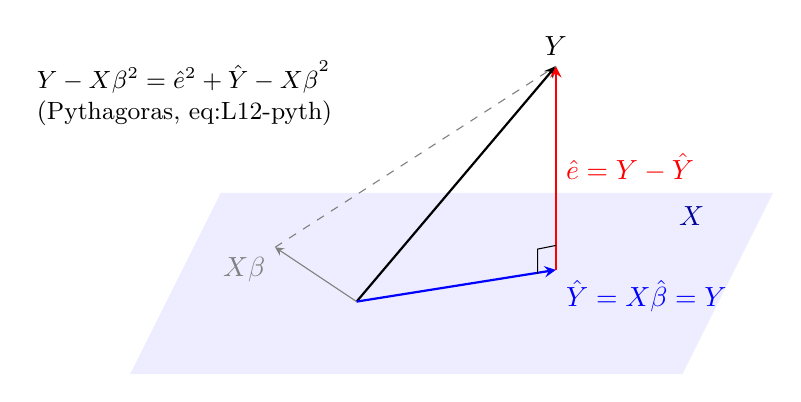
\begin{tikzpicture}[scale=1.15,>=stealth]
\fill[blue!7] (-2.5,-0.8) -- (3.6,-0.8) -- (4.6,1.2) -- (-1.5,1.2) -- cycle;
\node[blue!60!black] at (3.7,0.95) {$\colsp{X}$};
\coordinate (O) at (0,0);
\coordinate (P) at (2.2,0.35);
\coordinate (Y) at (2.2,2.6);
\coordinate (Q) at (-0.9,0.6);
\draw[->,thick] (O) -- (Y) node[above] {$Y$};
\draw[->,thick,blue] (O) -- (P) node[below right] {$\hat Y=X\hat\beta=\PX Y$};
\draw[->,thick,red] (P) -- (Y) node[midway,right] {$\hat e=Y-\hat Y$};
\draw[->,gray] (O) -- (Q) node[below left] {$X\beta$};
\draw[dashed,gray] (Q) -- (Y);
\draw (2.2,0.62) -- (2.0,0.58) -- (2.0,0.31);
\node[font=\small,align=left] at (-1.9,2.3) {$\pnorm{Y-X\beta}^2=\pnorm{\hat e}^2+\pnorm{\hat Y-X\beta}^2$\\(Pythagoras, \eqref{eq:L12-pyth})};
\end{tikzpicture}
\caption{Least squares geometry. $X\hat\beta$ is the foot of the perpendicular from $Y$ to the plane $\colsp{X}$. The residual $\hat e$ is orthogonal to $\colsp{X}$ (the normal equations), and every other $X\beta$ is farther from $Y$.}
\label{fig:L12-geometry}
\end{figure}

The name ``normal'' refers to this picture: the residual is \emph{normal} (perpendicular) to the
column space.

\begin{example}[Simple linear regression in matrix form]\label{ex:L12-slr}
Take $x=(1,2,3,4)$, $Y=(2,3,5,6)\T$ and $X=[\one,x]$ as in \cref{ex:L09-slr}. Then
\[
X\T X=\begin{pmatrix}4&10\\10&30\end{pmatrix},\qquad X\T Y=\begin{pmatrix}16\\47\end{pmatrix},\qquad
\det(X\T X)=120-100=20 .
\]
So
\[
\hat\beta=(X\T X)^{-1}X\T Y=\frac1{20}\begin{pmatrix}30&-10\\-10&4\end{pmatrix}\begin{pmatrix}16\\47\end{pmatrix}
=\frac1{20}\begin{pmatrix}480-470\\-160+188\end{pmatrix}=\begin{pmatrix}0.5\\1.4\end{pmatrix},
\]
exactly as in \cref{ex:L05-hand}, with $R_0^2=0.2$. Written out, the two normal equations
are $\sum_i\hat e_i=0$ and $\sum_ix_i\hat e_i=0$ (\cref{cor:L05-props}).
\end{example}

\begin{example}[A rank-deficient model: many solutions]\label{ex:L12-oneway}
One-way model, $k=2$, $n_1=n_2=2$, $\beta=(\mu,\mu_1,\mu_2)\T$ and data $Y=(3,5,8,10)\T$. With $X$ from
\cref{ex:L10-oneway}:
\[
X\T X=\begin{pmatrix}4&2&2\\2&2&0\\2&0&2\end{pmatrix},\qquad X\T Y=\begin{pmatrix}26\\8\\18\end{pmatrix}.
\]
The normal equations are $4\mu+2\mu_1+2\mu_2=26$, $2\mu+2\mu_1=8$, $2\mu+2\mu_2=18$. The first is the sum of the other
two, so they reduce to $\mu+\mu_1=4$ and $\mu+\mu_2=9$. The solution set is the line
\[
\hat\beta(t)=(t,\ 4-t,\ 9-t)\T,\qquad t\in\RR .
\]
Every $\hat\beta(t)$ gives the same fitted vector $X\hat\beta(t)=(4,4,9,9)\T$ (the group means), the same
residuals $(-1,1,-1,1)\T$, and $R_0^2=4$. The solution with the smallest norm minimises
$t^2+(4-t)^2+(9-t)^2$. Setting the derivative to zero gives $3t=13$, so $t=13/3$ and
$\hat\beta=(13/3,-1/3,14/3)\T$. This is the solution returned by the Moore--Penrose inverse (below).
\end{example}

\begin{note}[Supplementary: solutions via a generalized inverse]
A \vocab{generalized inverse} of a matrix $A$ is any matrix $\ginv A$ with $A\ginv AA=A$. Every matrix has one; the
Moore--Penrose inverse $A^{+}$ (\texttt{numpy.linalg.pinv}) is a particular choice. Then
\[
\hat\beta=\ginv{(X\T X)}X\T Y
\]
solves the normal equations. By \cref{lem:L12-colspace}, $X\T Y=X\T Xb$ for some $b$, so
$X\T X\,\ginv{(X\T X)}X\T Y=X\T X\,\ginv{(X\T X)}X\T Xb=X\T Xb=X\T Y$. With $A^{+}$ one gets the minimum-norm
solution of \cref{ex:L12-oneway}.
\end{note}

\subsection{Computation}
\nb{week04/L12\_normal\_equations.ipynb} solves the normal equations for both examples
(\texttt{numpy.linalg.solve} for full rank; \texttt{pinv} and \texttt{lstsq} for rank-deficient $X$). It
checks the Pythagorean identity \eqref{eq:L12-pyth} numerically, shows that different solutions give
the same fitted values, and compares with \texttt{statsmodels} OLS.

\subsection{Summary}
\begin{itemize}
  \item $\hat\beta$ is a least squares estimate iff it minimises $\pnorm{Y-X\beta}^2$ iff $X\T X\hat\beta=X\T Y$.
  \item Solutions always exist, because $X\T Y\in\colsp{X\T}=\colsp{X\T X}$. They are unique iff $\rank X=p$, in which case $\hat\beta=(X\T X)^{-1}X\T Y$.
  \item Pythagoras: $\pnorm{Y-X\beta}^2=\pnorm{Y-X\hat\beta}^2+\pnorm{X(\hat\beta-\beta)}^2$.
  \item The fitted values $X\hat\beta$ and the residuals are the same for every solution, and $X\T\hat e=0$.
\end{itemize}

\subsection{Exercises}
\begin{problem}\label{prob:L12-1}
Write the normal equations for $Y_i=\beta_1+\beta_2x_i+\eps_i$ in terms of $\sum x_i$, $\sum x_i^2$, $\sum Y_i$, $\sum x_iY_i$, and solve them to recover \cref{thm:L05-slr}.
\end{problem}
\begin{problem}\label{prob:L12-2}
For the one-way model with general $k$ and $n_i$, show that the normal equations reduce to $\mu+\mu_i=\bar Y_{i\cdot}$, $i=1,\dots,k$, and that $R_0^2=\SSW$.
\end{problem}
\begin{problem}\label{prob:L12-3}
Show that $\sum_i\hat e_i=0$ whenever $\one_n\in\colsp{X}$.
\end{problem}
\begin{problem}\label{prob:L12-4}
Verify that $G=\mathrm{diag}(0,\tfrac12,\tfrac12)$ is a generalized inverse of $X\T X$ in \cref{ex:L12-oneway}, and find the corresponding solution $GX\T Y$.
\end{problem}

\subsection{Further reading}
Christensen, \S2.2 (least squares estimation) and Appendix~B (generalized inverses); Rao, \S4a.2
(normal equations) and \S1b.5 (generalized inverse of a matrix).
